\section{Comparision between LNLT\_shell and NuShellX}
% Displaying the eigne values of each program side by side.
% comment on that we compute more states than nushellx computes.
% display the occupation numbers

To verify that the code descirbed in section \ref{sec:CodeExpl} works, several isotopes of oxygen was computed with LNLT\_shell and compared to the result from NuShellX with the usdb interaction. In table \ref{tab:ox18},\ref{tab:ox19} and \ref{tab:ox20} the eigenenergies of \(^{18,19,20}\rm{O}\) is compared to the values computed with NuShellX. The energies are relative the ground energy of \(^{16}\rm{O}\). There are almost no difference to the given numerical precission, only a few of the higher eigen-values differ slightly. In addition the code seems to correctly assign total angular momentum; the \(J_L\) columns are identical with the \(J_N\) columns. To illustrate the similarity further, the lowest energies are ploted in figure \ref{fig:ox18eig},\ref{fig:ox19eig} and \ref{fig:ox20eig}, where also a comparision to experiment is made.

\begin{figure}[ht!]
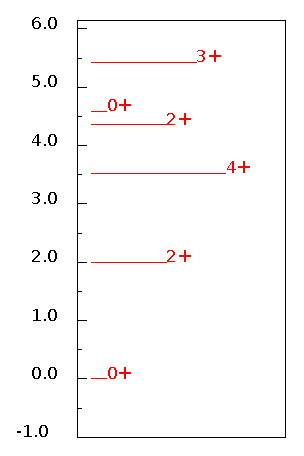
\includegraphics{ox18.eps}
\includegraphics[scale=0.56,trim=0cm 2.3cm 0cm 0cm]{o_18b.eps}
\caption{The lowest energy states of $^{18}\rm{O}$, computed by LNLT\_shell to the left compared to the eigenspectrum from experiment and NuShellX to the right}
\label{fig:ox18eig}
\end{figure}

\begin{figure}[ht!]
\includegraphics{ox19.eps}
\includegraphics[scale=0.56,trim=0cm 2.3cm 0cm 0cm]{o_19b.eps}
\caption{The lowest energy states of $^{19}\rm{O}$, computed by LNLT\_shell to the left compared to the eigenspectrum from experiment and NuShellX to the right}
\label{fig:ox19eig}
\end{figure}

\begin{figure}[ht!]
\includegraphics{ox20.eps}
\includegraphics[scale=0.56,trim=0cm 2.3cm 0cm 0cm]{o_20b.eps}
\caption{The lowest energy states of $^{20}\rm{O}$, computed by LNLT\_shell to the left compared to the eigenspectrum from experiment and NuShellX to the right}
\label{fig:ox20eig}
\end{figure}


In addition to the eigen-spectrum for each shell-occupation numbers where also computed. In tabel \ref{tab:ox18occ} all the shell-occupation numbers for all \(14\) states can be viewed, computed both with LNLT\_shell and with NuShellX. There are some slight difference, however this can be easily explained with that LNLT\_shell outputs higher precision than NuShellX does and thus the difference is moste likely due to rounding errors. In figure \ref{fig:occnum_lnlt} and \ref{fig:occnum_nushellx} the shell occupation for the ground state and the first excited states are visualized, computed by LNLT\_shell and NuShellX respectively. Also here there are a slight difference, which still can be explained with rounding errors. 

\begin{figure}
  \begin{center}
  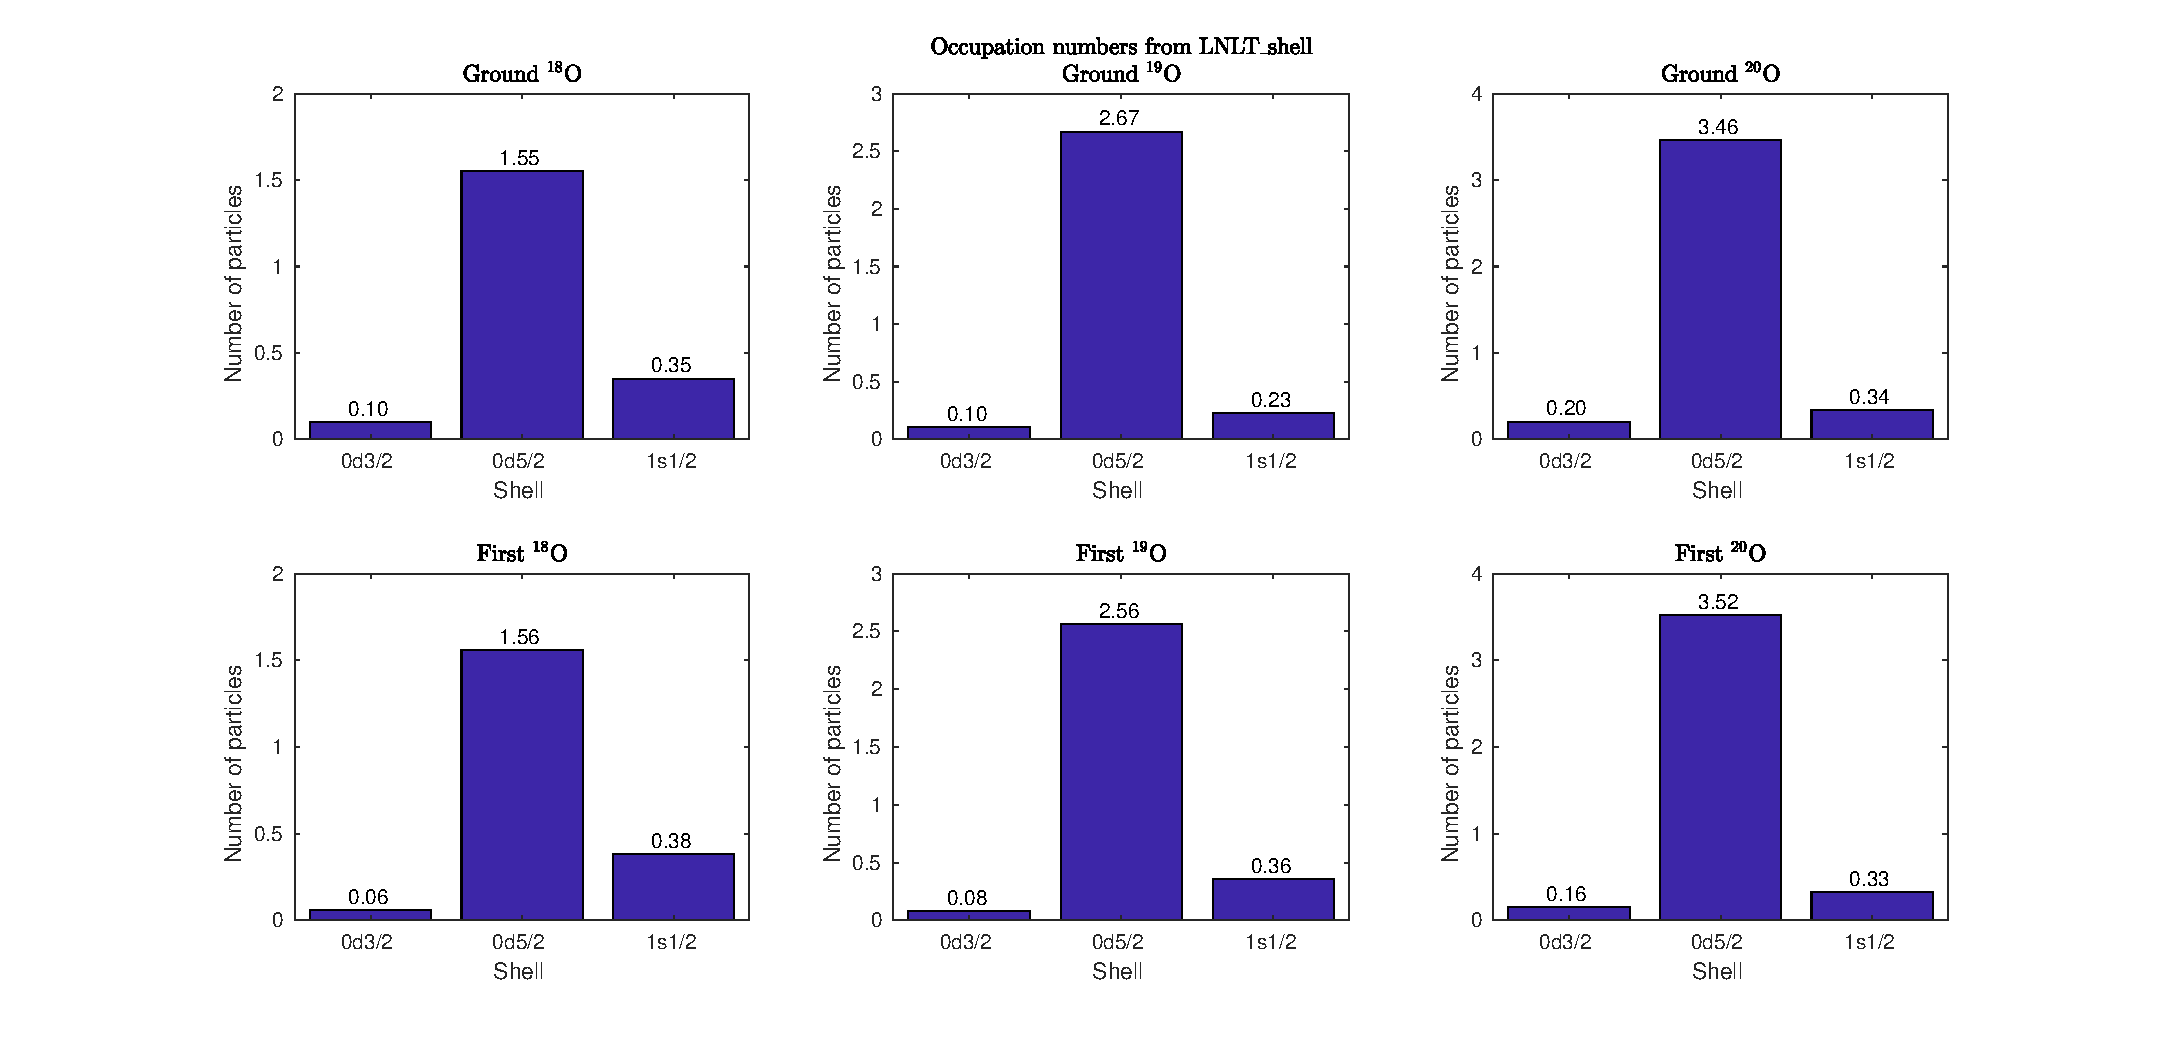
\includegraphics[scale=0.5]{occupation_numbers_lnlt.eps}
  \caption{The occupation numbers of the ground state and first excited state of \(^{18,19,20}\rm{O}\) as computed by LNLT\_shell.}
  \label{fig:occnum_lnlt}
  \end{center}
\end{figure}

\begin{figure}
  \begin{center}
  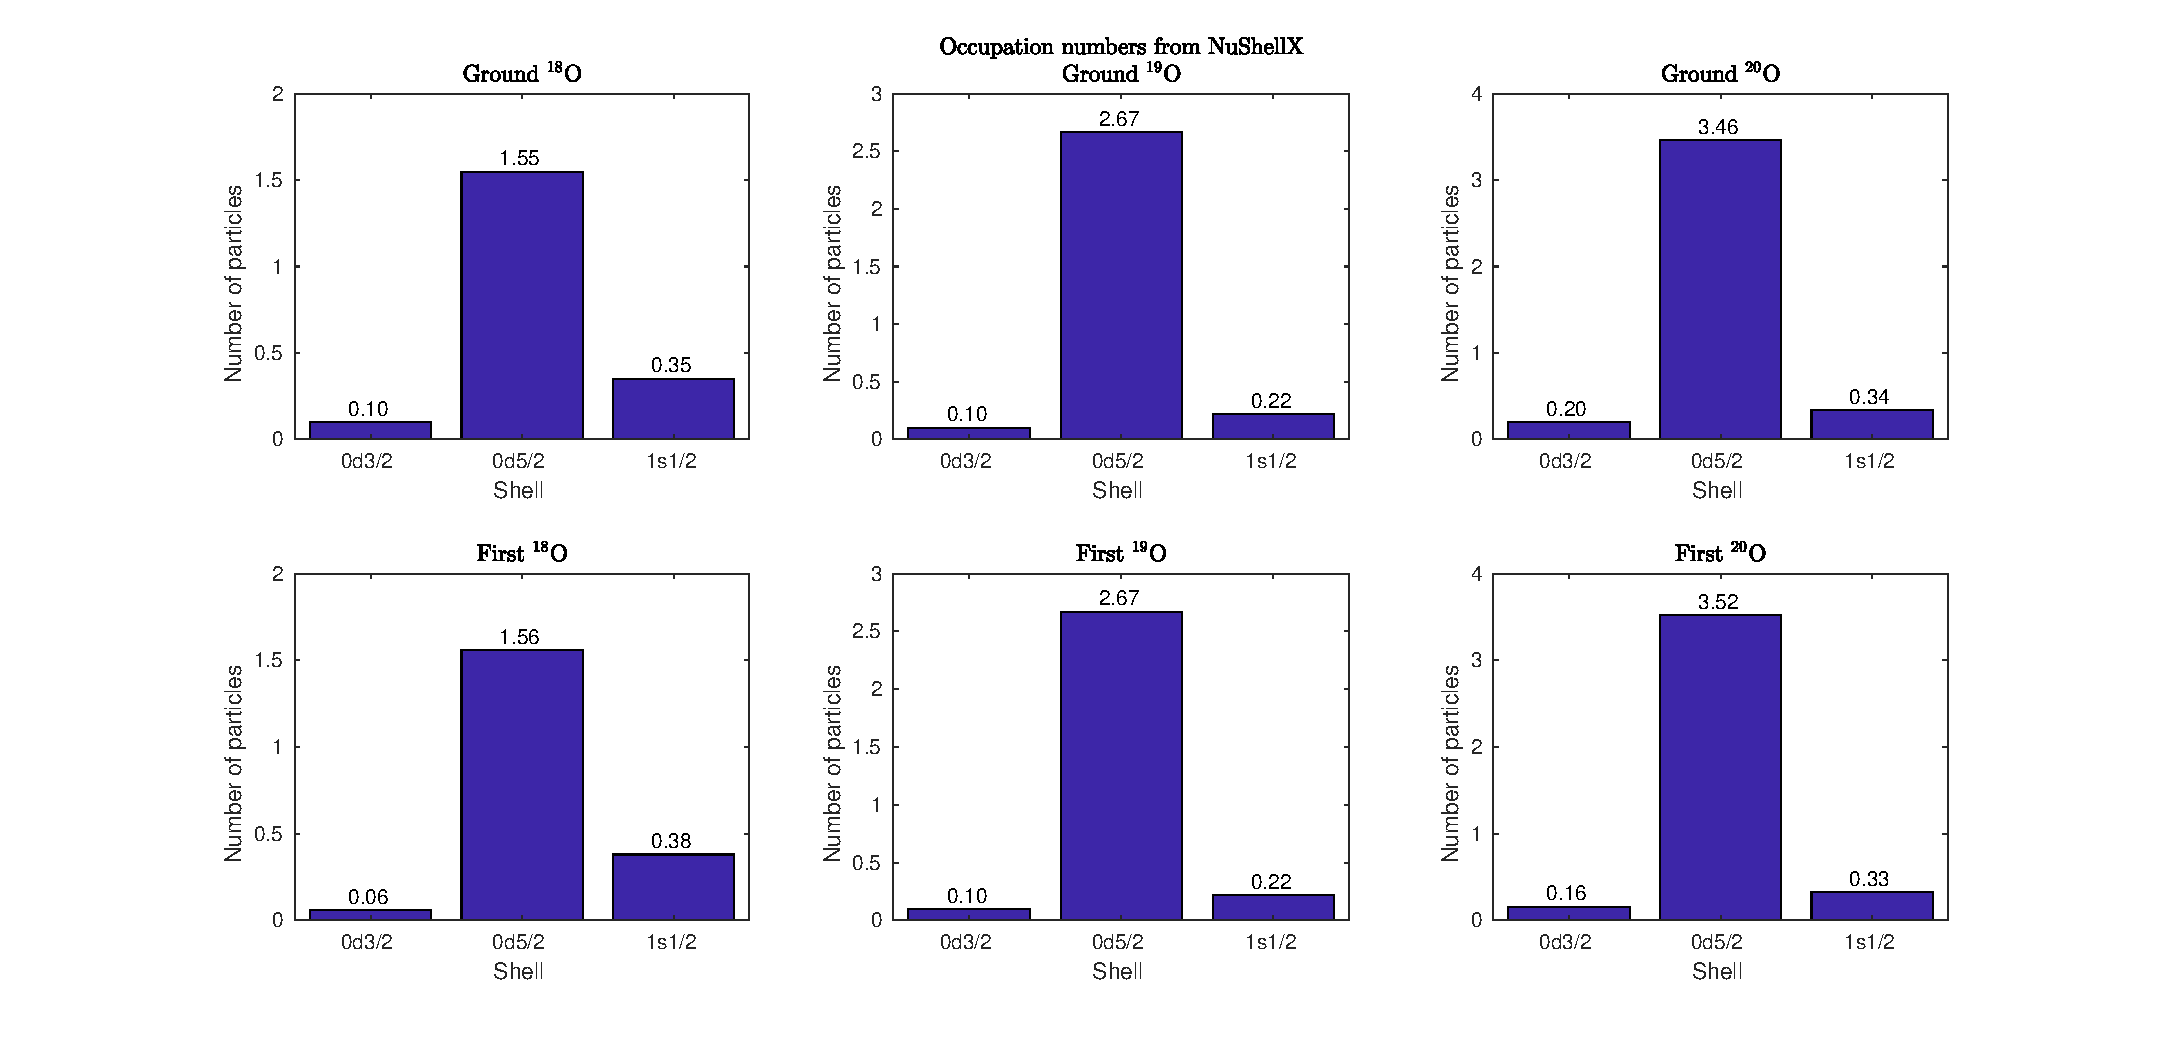
\includegraphics[scale=0.5]{occupation_numbers_nushellx.eps}
  \caption{The occupation numbers of the ground state and first excited state of \(^{18,19,20}\rm{O}\) as computed by NuShellX.}
  \label{fig:occnum_nushellx}
  \end{center}
\end{figure}

% Move the following tables to appendix.

\begin{table}[h]
\caption{The energy spectrum of $^{18}\rm{O}$ computed with LNLT\_shell (to the left) compared to NuShellX result (to the right). \(J_L\) is computed with LNLT\_shell while \(J_N\) are computed with NuShellX.}
\label{tab:ox18}
\begin{tabular}{|c|c|c|c|c|}
\hline Nr & \(E\) & \(J_{L}\) & \(E_{\rm{NuShellX}}\) & \(J_{N}\) \\
\hline 1   & -11.932 &       0 & -11.932 & 0 \\
\hline 2   &  -9.933 &       2 & -9.933 & 2 \\
\hline 3   &  -8.405 &       4 & -8.405 & 4 \\
\hline 4   &  -7.572 &       2 & -7.572 & 2 \\
\hline 5   &  -7.339 &       0 & -7.339 & 0 \\
\hline 6   &  -6.505 &       3 & -6.505 & 3 \\
\hline 7   &  -2.912 &       4 & -2.912 & 4 \\
\hline 8   &  -2.051 &       2 & -2.050 & 2 \\
\hline 9   &  -1.162 &       1 & -1.162 & 1 \\
\hline 10  &  -0.991 &       3 & -0.991 & 3 \\
\hline 11  &  -0.901 &       2 & -0.901 & 2 \\
\hline 12  &  -0.577 &       1 & -0.577 & 1 \\
\hline 13  &   3.077 &       0 & 3.077 & 0 \\
\hline 14  &   4.288 &       2 & 4.288 & 2 \\
\hline
\end{tabular}
\end{table}

\begin{table}[h]
\caption{The energy spectrum of $^{19}\rm{O}$ computed with LNLT\_shell (to the left) compared to NuShellX result (to the right). \(J_L\) is computed with LNLT\_shell while \(J_N\) are computed with NuShellX.}
\label{tab:ox19}
\begin{tabular}{|c|c|c|c|c||c|c|c|c|c|}
\hline Nr & \(E\) & \(J_{L}\) & \(E_{\rm{NuShellX}}\) & \(J_{N}\) & Nr & \(E\) & \(J_{L}\) & \(E_{\rm{NuShellX}}\) & \(J_{N}\) \\
\hline 1   & -15.956 &       5/2 & -15.956 & 5/2 & 20  &  -5.247 &       9/2 & -5.247 & 9/2 \\
\hline 2   & -15.838 &       3/2 & -15.838 & 3/2 & 21  &  -5.211 &       7/2 & -5.211 & 7/2 \\
\hline 3   & -14.389 &       1/2 & -14.389 & 1/2 & 22  &  -5.155 &       5/2 & -5.155 & 5/2 \\
\hline 4   & -13.586 &       9/2 & -13.586 & 9/2 & 23  &  -4.713 &       1/2 & -4.713 & 1/2 \\
\hline 5   & -13.072 &       7/2 & -13.072 & 7/2 & 24  &  -4.676 &       3/2 & -4.676 & 3/2 \\
\hline 6   &  -12.74 &       5/2 & -12.740 & 5/2 & 25  &  -4.001 &       5/2 & -4.002 & 5/2 \\
\hline 7   & -12.153 &       3/2 & -12.153 & 3/2 & 26  &  -3.379 &       3/2 & -3.379 & 3/2 \\
\hline 8   & -10.859 &       9/2 & -10.859 & 9/2 & 27  &  -3.348 &       7/2 & -3.348 & 7/2 \\
\hline 9   & -10.759 &       5/2 & -10.759 & 5/2 & 28  &  -1.363 &       5/2 & -1.363 & 5/2 \\
\hline 10  &  -9.875 &       3/2 & -9.875 & 3/2 & 29  &  -0.854 &       9/2 & -0.854 & 9/2 \\
\hline 11  &  -8.758 &       7/2 & -8.758 & 7/2 & 30  &  -0.392 &       7/2 & -0.392 & 7/2 \\
\hline 12  &  -8.095 &       1/2 & -8.095 & 1/2 & 31  &   0.105 &       1/2 & 0.105 & 1/2 \\
\hline 13  &  -8.088 &       5/2 & -8.095 & 1/2 & 32  &   0.755 &       1/2 & 0.755 & 1/2 \\
\hline 14  &   -7.97 &      11/2 & -7.970 & 11/2 & 33  &   1.401 &       3/2 & 1.401 & 3/2 \\
\hline 15  &  -7.118 &       3/2 & -7.118 & 3/2 & 34  &    1.41 &       5/2 & 1.401 & 3/2 \\
\hline 16  &    -6.5 &       7/2 & -6.500 & 7/2 & 35  &   1.689 &       5/2 & 1.689 & 5/2 \\
\hline 17  &  -6.361 &       5/2 & -6.361 & 5/2 & 36  &   2.037 &       3/2 & 2.037 & 3/2 \\
\hline 18  &  -6.184 &       9/2 & -6.184 & 9/2 & 37  &   5.946 &       3/2 & 5.946 & 3/2 \\
\hline 19  &  -5.597 &       3/2 & -5.597 & 3/2 &  -  &  -  &  -  &  -  &  -  \\
\hline
\end{tabular}
\end{table}

\begin{table}[h]
\caption{The energy spectrum of $^{20}\rm{O}$ computed with LNLT\_shell (to the left) compared to NuShellX result (to the right). \(J_L\) is computed with LNLT\_shell while \(J_N\) are computed with NuShellX.}
\label{tab:ox20}
\begin{tabular}{|c|c|c|c|c||c|c|c|c|c||c|c|c|c|c|}
\hline Nr & \(E\) & \(J_{L}\) & \(E_{\rm{NuShellX}}\) & \(J_{N}\) & Nr & \(E\) & \(J_{L}\) & \(E_{\rm{NuShellX}}\) & \(J_{N}\) & Nr & \(E\) & \(J_{L}\) & \(E_{\rm{NuShellX}}\) & \(J_{N}\) \\
\hline 1   & -23.632 &       0 & -23.632 & 0 & 29  & -11.122 &       2 & -11.122 & 2 & 57  &  -5.007 &       2 & -5.007 & 2 \\
\hline 2   & -21.886 &       2 & -21.886 & 2 & 30  &  -11.07 &       0 & -11.070 & 0 & 58  &  -4.906 &       0 & -4.906 & 0 \\
\hline 3   & -20.013 &       4 & -20.013 & 4 & 31  &  -10.93 &       4 & -10.930 & 4 & 59  &  -4.684 &       4 & -4.684 & 4 \\
\hline 4   & -19.478 &       2 & -19.478 & 2 & 32  & -10.714 &       4 & -10.714 & 4 & 60  &   -4.18 &       3 & -4.180 & 3 \\
\hline 5   & -18.518 &       1 & -18.518 & 1 & 33  & -10.544 &       3 & -10.544 & 3 & 61  &  -4.043 &       0 & -4.043 & 0 \\
\hline 6   & -18.475 &       2 & -18.475 & 2 & 34  & -10.451 &       1 & -10.450 & 1 & 62  &  -3.508 &       2 & -3.508 & 2 \\
\hline 7   & -18.363 &       4 & -18.363 & 4 & 35  & -10.305 &       6 & -10.305 & 6 & 63  &  -3.492 &       4 & -3.492 & 4 \\
\hline 8   &  -18.28 &       3 & -18.280 & 3 & 36  & -10.205 &       2 & -10.205 & 2 & 64  &   -3.23 &       3 & -3.230 & 3 \\
\hline 9   & -18.254 &       0 & -18.254 & 0 & 37  &  -9.862 &       2 & -9.862 & 2 & 65  &  -2.984 &       3 & -2.984 & 3 \\
\hline 10  & -16.248 &       4 & -16.248 & 4 & 38  &  -9.595 &       4 & -9.595 & 4 & 66  &  -2.953 &       1 & -2.953 & 1 \\
\hline 11  & -16.163 &       5 & -16.163 & 5 & 39  &  -9.533 &       3 & -9.533 & 3 & 67  &  -2.904 &       5 & -2.904 & 5 \\
\hline 12  & -15.455 &       2 & -15.455 & 2 & 40  &  -9.359 &       0 & -9.359 & 0 & 68  &  -2.885 &       2 & -2.885 & 2 \\
\hline 13  & -15.052 &       4 & -15.052 & 4 & 41  &  -9.141 &       1 & -9.141 & 1 & 69  &  -2.319 &       4 & -2.319 & 4 \\
\hline 14  & -14.996 &       2 & -14.996 & 2 & 42  &  -8.623 &       3 & -8.623 & 3 & 70  &  -2.228 &       2 & -2.228 & 2 \\
\hline 15  & -14.865 &       3 & -14.865 & 3 & 43  &  -8.549 &       2 & -8.549 & 2 & 71  &  -2.103 &       0 & -2.103 & 0 \\
\hline 16  & -13.963 &       0 & -13.963 & 0 & 44  &  -8.491 &       5 & -8.491 & 5 & 72  &  -1.114 &       1 & -1.114 & 1 \\
\hline 17  & -13.524 &       1 & -13.524 & 1 & 45  &  -8.186 &       2 & -8.186 & 2 & 73  &   -0.36 &       2 & -0.360 & 2 \\
\hline 18  &  -13.52 &       2 & -13.524 & 1 & 46  &  -7.814 &       3 & -7.814 & 3 & 74  &  -0.332 &       3 & -0.332 & 3 \\
\hline 19  & -13.241 &       6 & -13.241 & 6 & 47  &  -7.713 &       4 & -7.713 & 4 & 75  &   0.913 &       4 & 0.913 & 4 \\
\hline 20  & -13.229 &       3 & -13.229 & 3 & 48  &  -7.517 &       1 & -7.517 & 1 & 76  &   1.366 &       3 & 1.365 & 3 \\
\hline 21  & -12.508 &       2 & -12.508 & 2 & 49  &   -7.15 &       4 & -7.150 & 4 & 77  &   1.826 &       2 & 1.826 & 2 \\
\hline 22  & -12.314 &       5 & -12.314 & 5 & 50  &  -6.934 &       2 & -6.934 & 2 & 78  &   3.481 &       2 & 3.481 & 2 \\
\hline 23  & -12.231 &       1 & -12.231 & 1 & 51  &  -6.459 &       6 & -6.459 & 6 & 79  &   4.029 &       1 & 4.030 & 1 \\
\hline 24  & -11.991 &       5 & -11.991 & 5 & 52  &  -6.305 &       2 & -6.306 & 2 & 80  &   4.163 &       1 & 4.163 & 1 \\
\hline 25  & -11.849 &       1 & -11.849 & 1 & 53  &  -6.264 &       4 & -6.264 & 4 & 81  &   7.643 &       0 & 7.643 & 0 \\
\hline 26  & -11.637 &       4 & -11.637 & 4 & 54  &  -5.826 &       3 & -5.826 & 3 &  -  &  -  &  -  &  -  &  -  \\
\hline 27  & -11.426 &       3 & -11.426 & 3 & 55  &  -5.351 &       1 & -5.351 & 1 &  -  &  -  &  -  &  -  &  -  \\
\hline 28  & -11.267 &       3 & -11.267 & 3 & 56  &  -5.133 &       5 & -5.133 & 5 &  -  &  -  &  -  &  -  &  -  \\
\hline
\end{tabular}
\end{table}


\begin{table}[ht!]
\caption{The occupation numbers for \(^{18}\rm{O}\), computed with LNLT\_shell to the left and NuShellX to the right}
\begin{tabular}{|c|c|c|c|c|c|c|c|c|c|}
\hline State & $0d_{3/2}$ & $0d_{5/2}$ & $1s_{1/2}$ & Total & NuShellX & $0d_{3/2}$ & $0d_{5/2}$ & $1s_{1/2}$ & Total \\
\hline 1 & 0.098 & 1.552 & 0.35 & 2.0 & 1 & 0.1 & 1.55 & 0.35 & 2.0 \\
\hline 2 & 0.058 & 1.559 & 0.383 & 2.0 & 2 & 0.06 & 1.56 & 0.38 & 2.0 \\
\hline 3 & 0.063 & 1.937 & 0.0 & 2.0 & 3 & 0.06 & 1.94 & 0.0 & 2.0 \\
\hline 4 & 0.017 & 1.363 & 0.621 & 2.0 & 4 & 0.02 & 1.36 & 0.62 & 2.0 \\
\hline 5 & 0.003 & 0.353 & 1.644 & 2.0 & 5 & 0.0 & 0.35 & 1.64 & 1.99 \\
\hline 6 & 0.01 & 1.0 & 0.99 & 2.0 & 6 & 0.01 & 1.0 & 0.99 & 2.0 \\
\hline 7 & 0.937 & 1.063 & 0.0 & 2.0 & 7 & 0.94 & 1.06 & 0.0 & 2.0 \\
\hline 8 & 0.99 & 0.942 & 0.068 & 2.0 & 8 & 0.99 & 0.94 & 0.07 & 2.0 \\
\hline 9 & 1.0 & 0.994 & 0.006 & 2.0 & 9 & 1.0 & 0.99 & 0.01 & 2.0 \\
\hline 10 & 0.99 & 1.0 & 0.01 & 2.0 & 10 & 0.99 & 1.0 & 0.01 & 2.0 \\
\hline 11 & 0.958 & 0.116 & 0.926 & 2.0 & 11 & 0.96 & 0.12 & 0.93 & 2.01 \\
\hline 12 & 1.0 & 0.006 & 0.994 & 2.0 & 12 & 1.0 & 0.01 & 0.99 & 2.0 \\
\hline 13 & 1.899 & 0.095 & 0.007 & 2.0 & 13 & 1.9 & 0.09 & 0.01 & 2.0 \\
\hline 14 & 1.977 & 0.021 & 0.002 & 2.0 & 14 & 1.98 & 0.02 & 0.0 & 2.0 \\
\hline
\end{tabular}
\end{table}
